\clearpage

\chapter*{\textbf{Anhang}}\label{appendix}
\addcontentsline{toc}{chapter}{\textbf{Anhang}}
\markboth{\textbf{Anhang}}{\textbf{Anhang}}

\section*{A: Fragebogen}

\subsection*{A.1 Instrumente und Skalen}

Der eingesetzte Fragebogen bestand aus fünf Blöcken. Die Implementierung findet sich in\linebreak \texttt{evaluation/page.tsx}, die deutschen Wortlaute in \texttt{messages/de.json}.

\begin{enumerate}
    \item \textbf{Vorerfahrung \& Selbsteinschätzung:} Altersgruppe, Beschäftigungsstatus, IT/Software-Hintergrund, Programmierkenntnisse (Skala 1--5), Selbstwirksamkeit (3 Items, Likert 1--7)
    \item \textbf{Cognitive Load:} Mentale Anstrengung (Paas-Skala, 1--9), Frustration (NASA-TLX-Teilska\-la, 0--100)
    \item \textbf{Systemqualität:} SUS (10 Items, Likert 1--5), UEQ-S (8 Gegensatzpaare, 1--7)
    \item \textbf{KI-Assistent (nur Gruppe~B):} Nützlichkeit (3 Items), Vertrauen (3 Items, darunter ein invertiertes Item)
    \item \textbf{Abschluss:} Net Promoter Score (0--10), offenes Freitext-Feedback (Pflichtfeld)
\end{enumerate}

\subsection*{A.2 Beispielhafte Original-Items (Deutsch)}

\textbf{SUS-Beispiele:}
\begin{itemize}
    \item Ich denke, dass ich das System gerne häufig benutzen würde.
    \item Ich fand das System einfach zu benutzen.
    \item Ich fühlte mich bei der Benutzung des Systems sehr sicher.
\end{itemize}

\textbf{UEQ-S Gegensatzpaare (Auszug):}
\begin{itemize}
    \item behindernd $\leftrightarrow$ unterstützend
    \item kompliziert $\leftrightarrow$ einfach
    \item langweilig $\leftrightarrow$ spannend
    \item konventionell $\leftrightarrow$ neuartig
\end{itemize}

\textbf{Cognitive-Load-Items:}
\begin{itemize}
    \item Wie viel geistige Anstrengung mussten Sie aufbringen, um die Aufgaben zu lösen? (Paas, 1--9)
    \item Wie unsicher, entmutigt, irritiert oder gestresst fühlten Sie sich während der Aufgaben? (NASA-TLX Frustration, 0--100)
\end{itemize}

\section*{B: Ausgewählte Drill-Aufgaben (Beispiele)}

Die folgenden Beispiele entstammen dem statischen Drill-Pool (\texttt{src/courses/\\pythonDrillTasks.ts}) und repräsentieren die zwei eingesetzten Aufgabentypen.

\subsection*{B.1 Multiple-Choice-Aufgabe: Konzeptabfrage}

\textbf{ID:} \texttt{mcq-print-1} \\
\textbf{Frage:} Was macht die \texttt{print()}-Funktion? \\
\textbf{Antwortoptionen:}
\begin{itemize}
    \item Speichert Daten auf der Festplatte
    \item \textbf{Gibt Text in der Konsole aus} \textrm{(korrekt)}
    \item Erstellt eine Variable
    \item Rechnet Zahlen aus
\end{itemize}

\subsection*{B.2 Multiple-Choice-Aufgabe: Output vorhersagen}

\textbf{ID:} \texttt{mcq-print-3} \\
\textbf{Aufgabe:} Welche Ausgabe erzeugt der folgende Code?
\begin{verbatim}
print('Python')
print('Lernen')
\end{verbatim}
\textbf{Korrekte Antwort:} \texttt{Python} (Zeile 1), \texttt{Lernen} (Zeile 2)

\subsection*{B.3 Code-Drill: Schreiben}

\textbf{ID:} \texttt{code-print-1} \\
\textbf{Titel:} Text ausgeben \\
\textbf{Aufgabenstellung:} Gib den Text \texttt{'Willkommen'} in der Konsole aus. Nutze \texttt{print()} direkt mit dem Text -- du brauchst keine Variable. \\
\textbf{Starter-Code:}
\begin{verbatim}
# Schreibe hier deinen Code
\end{verbatim}
\textbf{Erwartete Ausgabe:} \texttt{Willkommen}

\section*{C: Beispiel-Prompts für die KI-Generierung}

Die folgenden Auszüge dokumentieren die Kernprinzipien der eingesetzten Systemprompts. Da die vollständigen Prompts mehrere hundert Token umfassen, werden hier nur die strukturellen Prinzipien zusammengefasst. Die vollständigen Prompt-Texte sind im Quellcode des Projekts einsehbar (vgl.\ Anhang~D, Repository-Link).

\subsection*{C.1 Systemprompt: KI-Tutor (Lernassistenz)}

\textbf{Datei:} \texttt{src/actions/openaiChatActionV3.ts} \\

\noindent Kernprinzipien des Prompts:
\begin{itemize}
    \item Rolle: hilfreicher KI-Assistent für das Python-Bootcamp
    \item Didaktisches Prinzip: keine direkte Komplettlösung, sondern schrittweise, progressive Hinweise
    \item Strikte Ausgabeformatierung: strukturiertes JSON mit den Typen \texttt{text}, \texttt{admonition} und \texttt{codeblock}
    \item Kontextinjek\-tion: aktuelle Aufgabe, Startercode, Konsolenausgabe, Hint-Level und Benutzerprofilierung werden je Anfrage als Nutzerkontext übergeben
    \item Hint-Eskalation: mit jeder Anfrage wird eine Stufe weiter eskaliert; Solution-Strings werden erst ab Level~5 mitgesendet
\end{itemize}

\subsection*{C.2 Systemprompt: KI-gestützte Drill-Auswahl (Pool-basiert)}

\textbf{Datei:} \texttt{src/actions/aiDrillSelectionFromPoolAction.ts} \\

\noindent Kernprinzipien des Prompts:
\begin{itemize}
    \item Auswahl einer didaktisch passenden Kombination aus einer MCQ- und einer Code-Aufgabe aus dem statischen Pool
    \item Performance-adaptive Schwierigkeit: Fehlerhistorie und Erfolgsrate der lernenden Person werden übergeben
    \item Priorisierung noch nicht gezeigter Aufgaben (\texttt{timesShown = 0})
    \item Keine Wiederholung bereits korrekt gelöster Drills
    \item Strukturierte Ausgabe über striktes JSON-Schema (\textit{Structured Outputs}, \texttt{strict: true})
\end{itemize}

\section*{D: Screenshots der Web-Anwendung und Verfügbarkeit der Daten}\label{appendix:daten}

Der vollständige Quellcode des Lernsystems sowie alle anonymisierten Studiendaten (Chat-Verläufe, Aufgaben-Log-Daten, Fragebogenantworten) sind öffentlich zugänglich unter:

\begin{center}
\url{https://github.com/Shaco74/4CID-Adaptive-Python-Tutor}
\end{center}

Die folgenden Abbildungen zeigen die wichtigsten Ansichten der implementierten Lernplattform.

\begin{figure}[htbp]
    \centering
    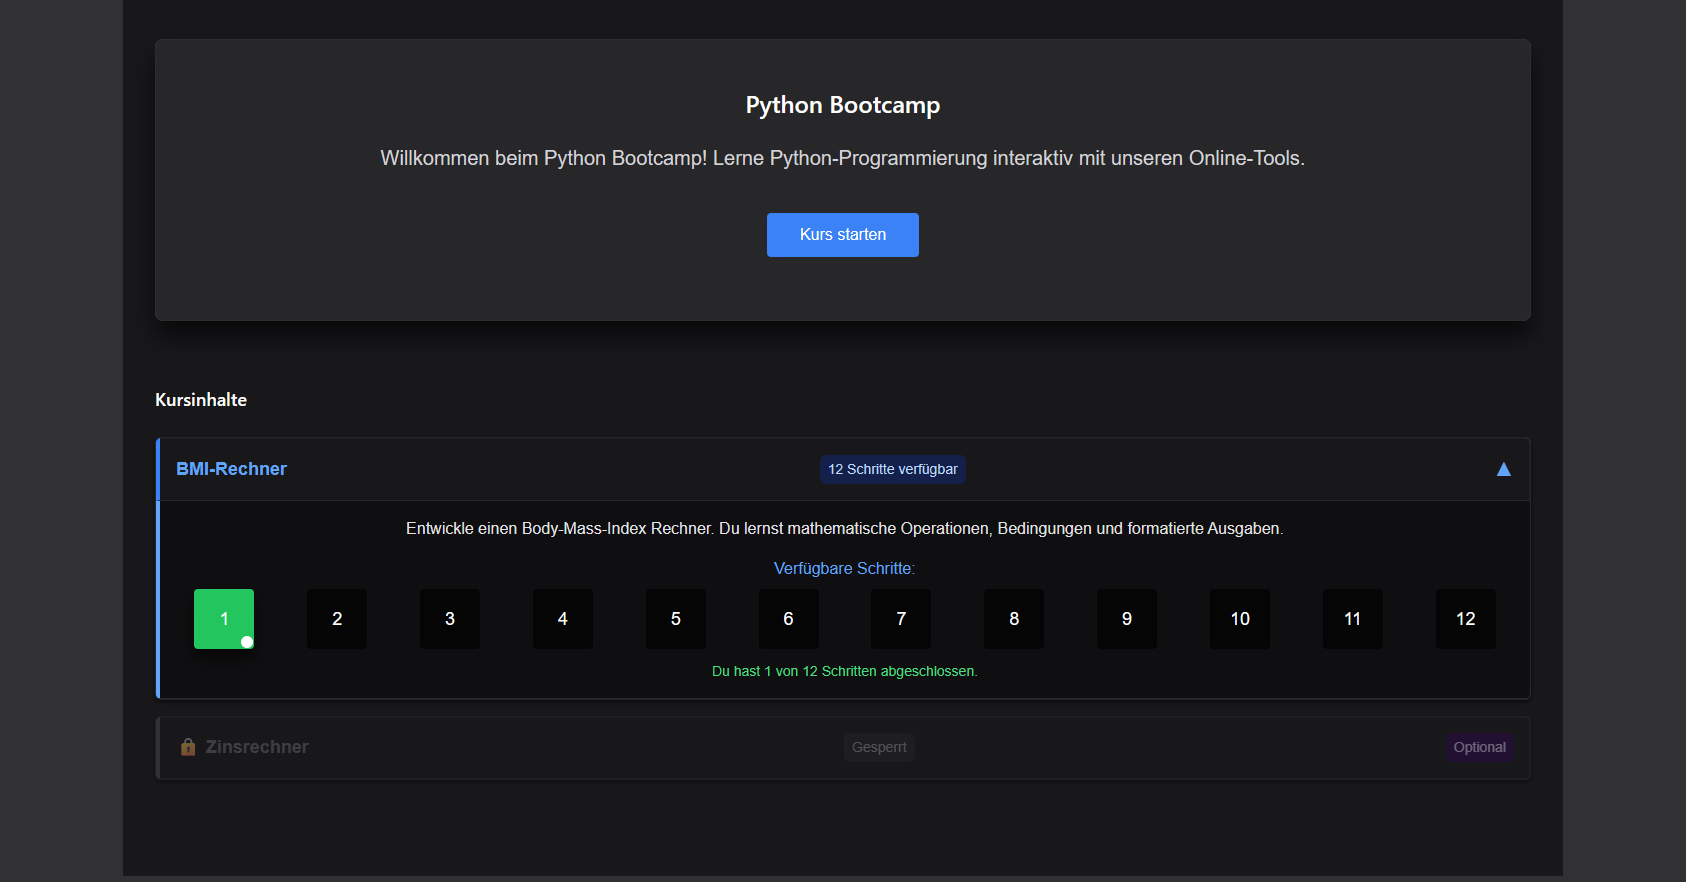
\includegraphics[width=0.80\textwidth]{pic/bilder-der-app/home-kursuebersicht}
    \caption{Dashboard mit Kursübersicht. Abgeschlossene Schritte werden grün hervorgehoben; der Zinsrechner ist als optionaler Aufbaukurs gesperrt, bis der BMI-Rechner abgeschlossen wurde.}
    \label{fig:anhang_dashboard}
\end{figure}

\begin{figure}[htbp]
    \centering
    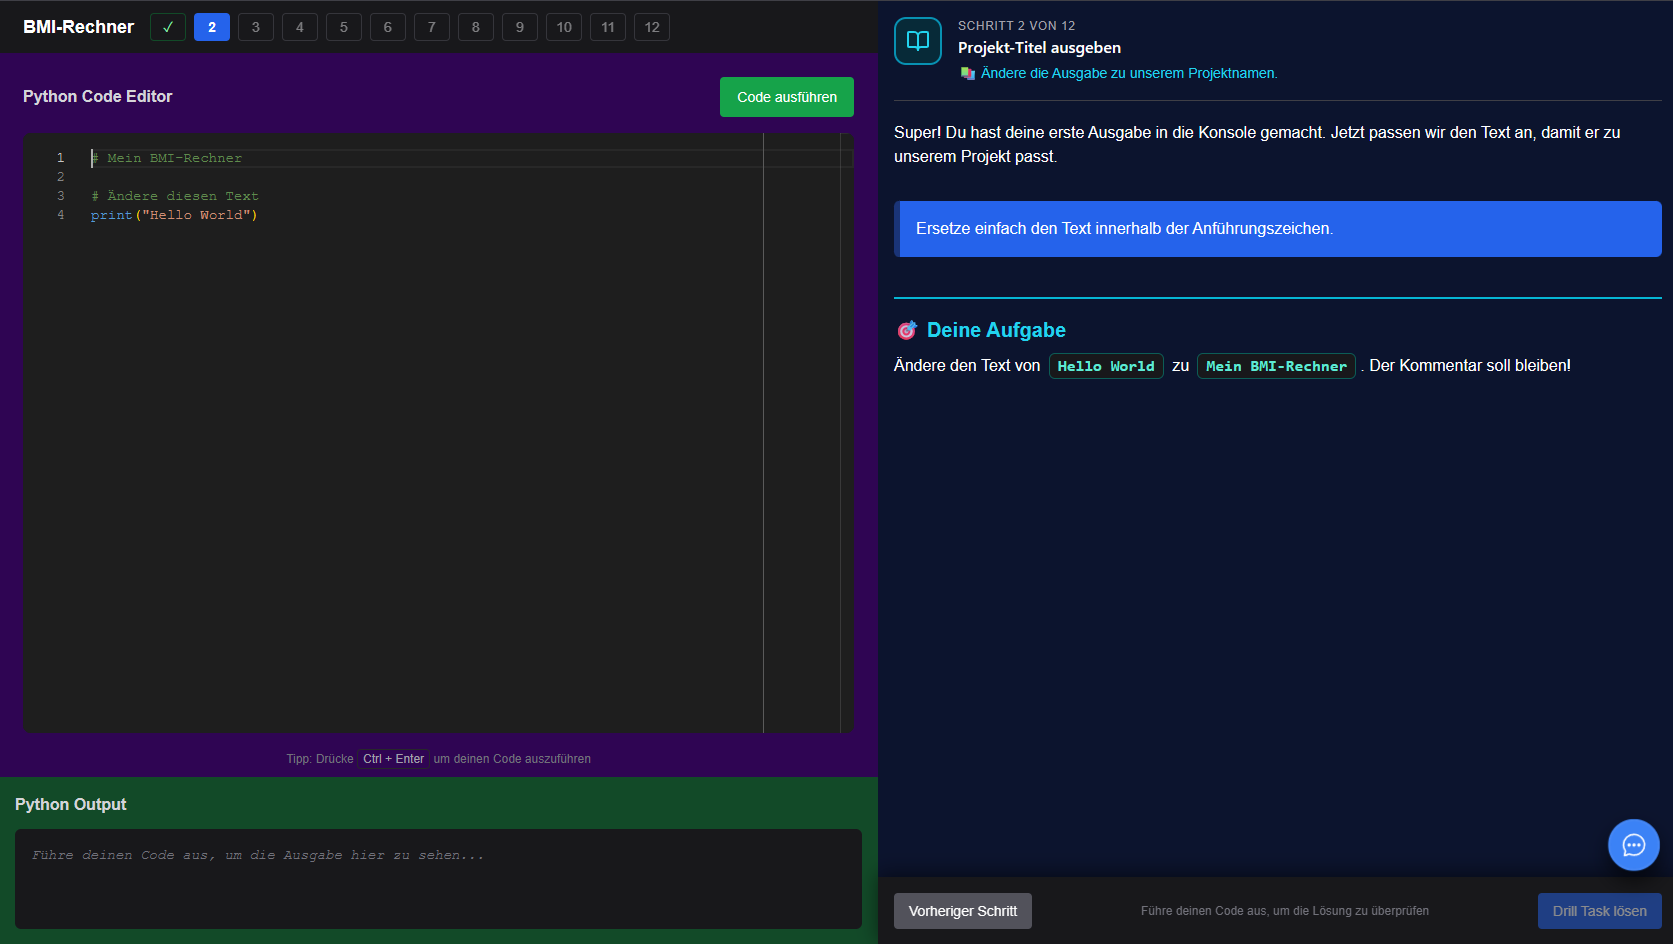
\includegraphics[width=0.75\textwidth]{pic/bilder-der-app/kursansicht-full}
    \caption{Kursansicht (Schritt~1 von 12): Links der Monaco-Code-Editor mit Startercode und Python-Ausgabebereich, rechts die Aufgabenstellung mit farbigen Hinweisboxen. Der blaue Chat-Button (roter Pfeil) öffnet den KI-Tutor (nur Gruppe~B).}
    \label{fig:anhang_kursansicht}
\end{figure}

\begin{figure}[htbp]
    \centering
    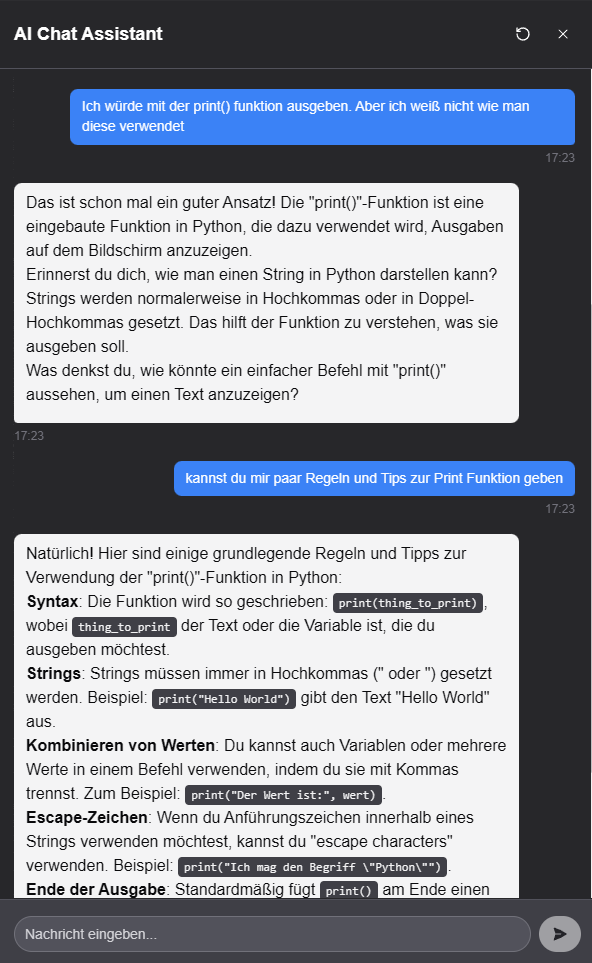
\includegraphics[width=0.75\textwidth]{pic/bilder-der-app/chat-beispiel}
    \caption{KI-Tutor-Chat (Gruppe~B): Das progressive Hint-System antwortet auf eine Frage zur \texttt{print()}-Funktion mit Rückfragen statt direkter Lösung.}
    \label{fig:anhang_chatverlaeufe}
\end{figure}

\begin{figure}[htbp]
    \centering
    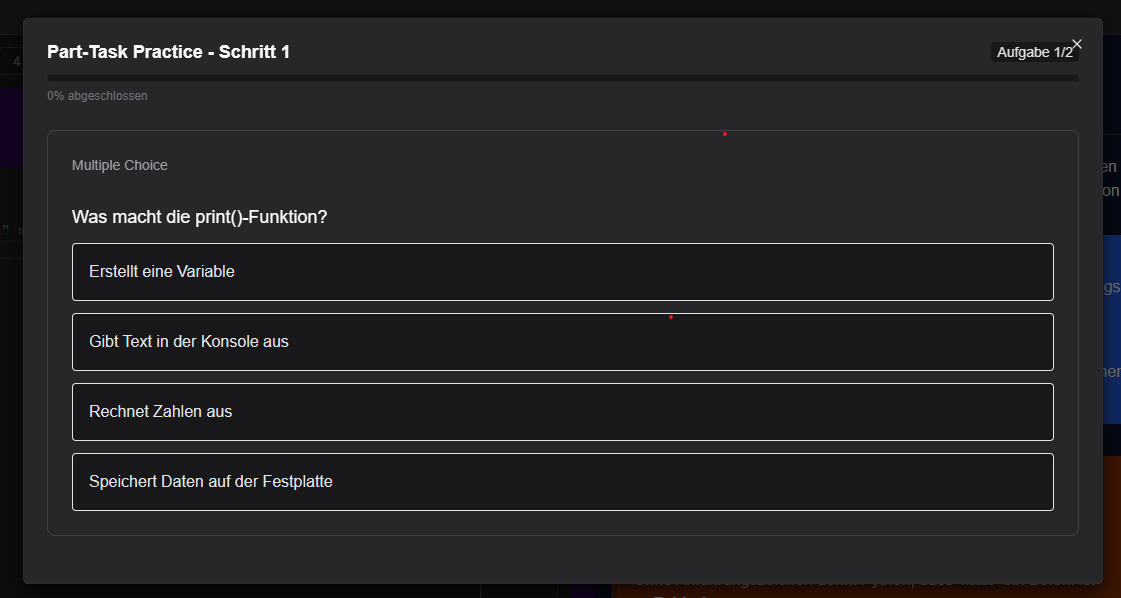
\includegraphics[width=0.75\textwidth]{pic/bilder-der-app/drill-multiple-choice}
    \caption{Part-task Practice -- Multiple-Choice-Aufgabe (Schritt~1): Konzeptabfrage zur \texttt{print()}-Funktion aus dem statischen Drill-Pool.}
    \label{fig:anhang_drill_mcq}
\end{figure}

\begin{figure}[htbp]
    \centering
    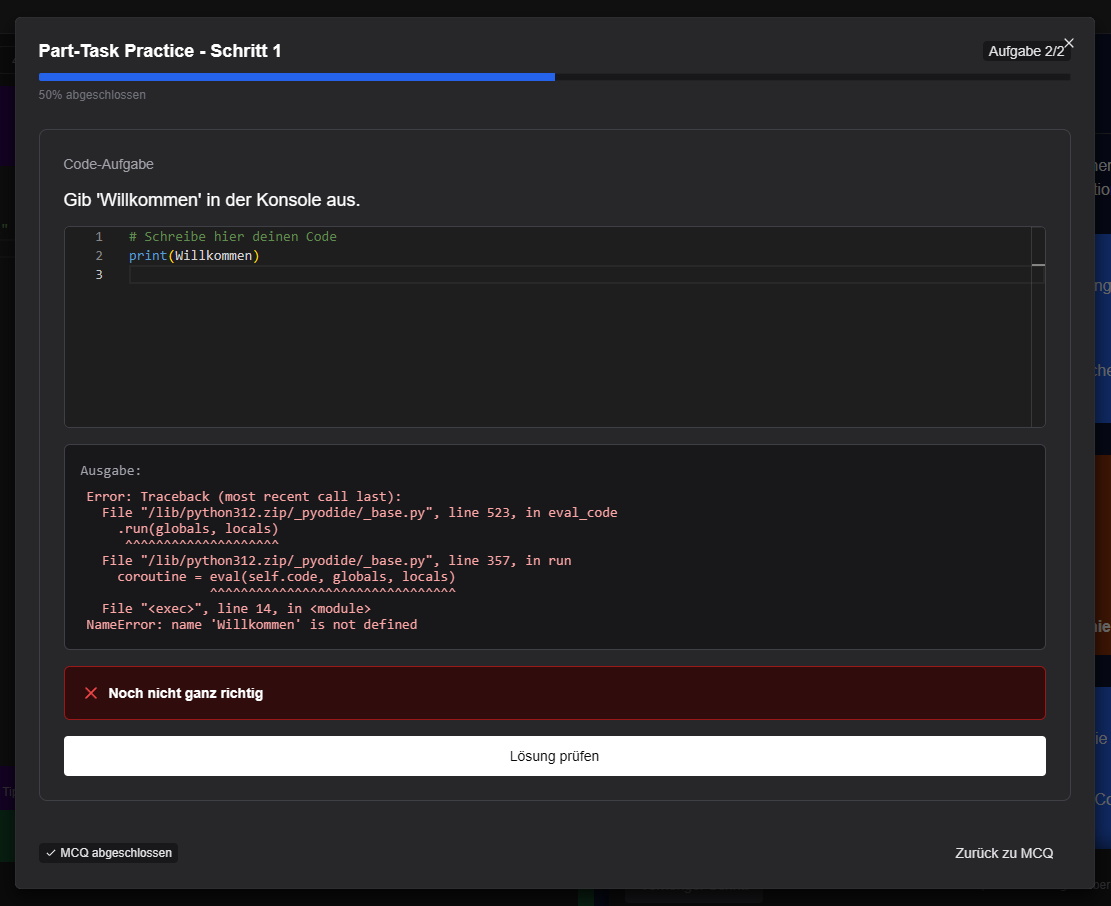
\includegraphics[width=0.75\textwidth]{pic/bilder-der-app/drill-code-aufgabe}
    \caption{Part-task Practice -- Code-Aufgabe (Schritt~1): Die Lernende hat \texttt{Willkommen} ohne Anführungszeichen eingegeben; das System zeigt den Python-Fehler und meldet die Lösung als noch nicht korrekt.}
    \label{fig:anhang_drill_code}
\end{figure}

\clearpage
\section*{E: Werkzeug- und KI-Protokoll}

Nachfolgend sind alle wesentlichen digitalen Werkzeuge und KI-Systeme aufgeführt, die bei der Erstellung dieser Arbeit zum Einsatz kamen.
Die Auflistung folgt der Empfehlung des Betreuers, alle verwendeten Hilfsmittel transparent auszuweisen.

\renewcommand{\arraystretch}{1.4}
\begin{table}[htbp]
\centering
\caption{Protokoll der verwendeten Werkzeuge und KI-Systeme}
\label{tab:werkzeugprotokoll}
% reduce inter-column padding and slightly smaller font to help fit columns
\begingroup
	\setlength{\tabcolsep}{6pt}% adjust if necessary
	\small
	\begin{tabular}{|P{3.2cm}|P{2.6cm}|P{4.6cm}|P{3.8cm}|}
	\hline
	\textbf{Werkzeug / System} & \textbf{Version / Zeitraum} & \textbf{Einsatzbereich} & \textbf{Validierung} \\
	\hline
	GitHub Copilot (Microsoft) mit GPT-4o, GPT-5.1 sowie Claude~Sonnet~4.6 \& Claude~Opus~4.6 (Anthropic) &
	Copilot in VS~Code, Juni~2025--Mrz.~2026 &
	Formulierungsvorschläge, Gliederungsstruktur, \LaTeX-Syntax, Erarbeitung von Kapitelgerüsten und Leitfragen, Code-Generierung und -Analyse, BibTeX-Bereinigung; KI-Unterstützung bei der Entwicklung der Lernplattform-Codebase &
	Alle Ausgaben manuell geprüft und inhaltlich angepasst; Quellen und DOIs separat veri\-fiziert \\
	\hline
	Visual Studio Code \cite{vscode} mit LaTeX Workshop Extension &
	VS~Code~1.x, Feb.--Mrz.~2026 &
	Entwicklungsumgebung für \LaTeX-Ausarbeitung und Programmierprototyp; Build, Formatierung, PDF-Vorschau &
	Kein KI-Einsatz; reines Editierwerkzeug \\
	\hline
	latexmk / \TeX~Live (WSL) &
	\TeX~Live~2024, Feb.--Mrz.~2026 &
	Kompilierung der \LaTeX-Arbeit zu PDF &
	Kein KI-Einsatz \\
	\hline
	OpenAI API (gpt-4o-mini) \cite{openai_api} &
	API, Jan.--Mrz.~2026 &
	KI-Tutor und Aufgabenauswahl im entwickelten Lernprototyp (Forschungsgegenstand der Arbeit) &
	Prototyp-intern; Ausgaben im Rahmen der Studie erhoben und ausgewertet \\
	\hline
	\end{tabular}
\endgroup
\end{table}

\noindent
\textit{Anmerkung:} Triviale Werkzeuge (Browser, Datei\-ver\-wal\-tung) sind gemäß den Hinweisen des Betreuers nicht gesondert aufgeführt.
Die inhaltliche Verantwortung für alle Aussagen, Interpretationen und Schlussfolgerungen liegt beim Autor.
